\documentclass[10pt,a4paper]{article}
\usepackage[utf8]{inputenc}
\usepackage[spanish]{babel}
\usepackage{amsmath}
\usepackage{amsfonts}
\usepackage{amssymb}
\usepackage{graphicx}
\usepackage{listings}

\lstset{basicstyle=\footnotesize, language=sql}

\author{César Bolívar Severino, Pedro Gallardo Robinson} % Porqué no sale esta wea en el pdf?
														   % coz you have to do maketitle :DDDD
														   % wena xD
\title{Fase III}


\begin{document}

\maketitle

\section{Descripción}

La base de datos de música tiene novedosas funcionalidades que pueden resultar muy prácticas a la hora de obtener información relevante, tanto de los artistas, como de las canciones o álbumes.
Su característica mas reciente, es la capacidad de encontrar diferentes versiones de la misma canción, ya que tiene registro de las composiciones originales (pudiendo ser ésta la primera versión de una canción, tanto como una pieza escrita por algún músico clásico antiguo).
\newline
Se han cambiado algunos enfoques desde la fase pasada.
\begin{enumerate}
	\item Ahora todos los artistas son tratados como bandas y están compuestos por personas, los solistas son casos especiales de bandas compuestas por una sola persona.
	\item Se han puestos \textit{numeros de identificación} (nombrados como \textit{id} en las relaciones), con la finalidad de normalizar de manera sencilla los datos y evitar cambios complicados en las tablas de relaciones.
\end{enumerate}

\newpage

\section{Modelo Conceptual}

\subsection{MER}
\begin{center}
\includegraphics[scale=0.25]{MER.png}
\end{center}

\subsection{Restricciones Adicionales}
 %Escribir restricciones adicionales acá.
 \begin{enumerate}
 \item Un integrante de una banda no podrá salir ni entrar dos veces seguidas, por consecuente, las fecha de salida debe ir después de una fecha de entrada y no podrá entrar antes de una fecha de salida.
 \item
 \end{enumerate}
\newpage

\section{Modelo Relacional}

\subsection{Export Postgres}
%\lstinputlisting[language=Sql]{export_postgres.sql}

\subsection{Dependencias funcionales}
%Agregar Dependencias funcionales acá.
Se han definido las siguientes dependencias funcionales para cada entidad del modelo.
\begin{description}

	\item [Persona]
	%\newline
	$	\{ dni, pais\_nacimiento \} \rightarrow \{ nombre, apellido, sexo, fecha\_nacimiento \} $

	\item [Artista]
	%\newline
	$	\{ id \} \rightarrow \{ nombre\_artistico, pais\_consagracion \} $

	\item [Canción]
	%\newline
		$\{ id\_cancion \} \rightarrow \{ nombre, id\_artista \}$

	\item [Composición]
	%\newline
	$\{ id\_cancion \} \rightarrow \{ nombre\_tema, id\_artista, duracion, fecha\_lanzamiento, id\_composicion \}$

	\item [Album]
	%\newline
	$\{ id\_album \} \rightarrow \{ nombre\_album, fecha\_lanzamiento, sello\_discografico \}$

	\item [Instrumento]
	$\{ id\} \rightarrow \{nombre\_instrumento\} $

	\item [Pais]
	$ \{nombre\_pais\} \rightarrow \{continente\} $

	\item [ComposicionArtista]
	$ \{dni\_persona, pais\_persona, id\_artista \} \rightarrow \{ fecha\_ingreso \} $

	%%%%%
	\item [Compuesta]
	$ \{dni, pais\_origen, artista \} \rightarrow \{ fecha\_ingreso \} $

	\item [FechaSalida]
	$ \{dni, pais\_origen, artista \} \rightarrow \{ fecha\_salida \} $

	\item [Pertenece]
	$ \{id\_cancion, artista, nombre \} \rightarrow \{ numero\_pista \} $
		
\end{description}

\newpage

\section{Consultas}
% Hacer esta sección más bonita plz

\subsection{Consulta 1}
Obtener el nombre y apellido de todos los guitarristas estadounidenses.

\begin{lstlisting}
select p.nombre, p.apellido
from Persona as p, Instrumento as i, TocaInstrumento as ti
where p.dni = ti.dni and p.pais_nacimiento = ti.pais_origen
	and i.id = ti.instrumento and i.nombre = 'Guitarra electrica'
\end{lstlisting}

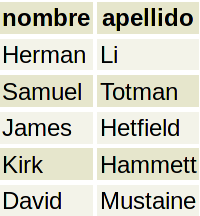
\includegraphics[scale=0.35]{resultado_consulta_1.png}


\subsection{Consulta 2}
Obtener el nombre de todos los artistas que hayan lanzado albumes bajo Roadrunner Records, junto con dichos albumes.

\begin{lstlisting}
select ar.nombre_artistico, al.nombre
from Artista as ar, Album as al, Lanza as l
where ar.id = l.artista and al.id = l.album and
	al.sello = 'Roadrunner Records'
\end{lstlisting}


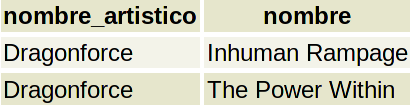
\includegraphics[scale=0.35]{resultado_consulta_2.png}


\subsection{Consulta 3}
Obtener el nombre y album al que pertenecen todas las canciones de Nujabes.

\begin{lstlisting}
select i.nombre, al.nombre
from Interpretacion as i, Album as al, Pertenece as p, Artista as ar
where p.id_cancion = i.id_cancion and p.artista = i.id_artista
	and p.nombre = i.nombre and p.album = al.id and p.artista = ar.id
	and ar.nombre_artistico = 'Nujabes'
\end{lstlisting}

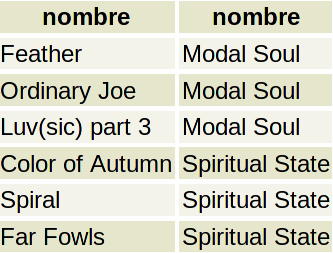
\includegraphics[scale=0.35]{resultado_consulta_3.png}

%%%
%% OBS: omití tildes en las consultas porque da problemas con el encoding
%%%
\end{document}
